\begin{pastexam}[label={px:df3-109-ds-04}]{地方三等資訊處理 109 年 第四題}
（申論；24 分）

\begin{itemize}[leftmargin=2.2em]
\item[㈠] 在一棵高度為 h(h=0,1,2,\ldots)的 AVL tree 中：(1)高度為6之 AVL tree 最多可能有幾個 nodes？最少可能
有幾個 nodes？（假設 root 之 h=0）（6分）(2)假設此樹共有45個 nodes。請問此 AVL tree 可能最高之高度及最矮之
高度各為何？（6分）
\item[㈡] 請將下列數字\{17, 60, 24, 5, 7\}逐步插入圖1的 AVL tree 中，並平衡之。（12分）
\end{itemize}
\begin{center}
\begin{tikzpicture}[v/.style={ellipse,draw,minimum width=9mm,minimum height=6mm,inner sep=0pt,font=\small},
    level distance=11mm, level 1/.style={sibling distance=26mm}, level 2/.style={sibling distance=16mm}]
\node[v] {14}
  child {node[v] {8} child {node[v] {4}} child[missing] {}}
  child {node[v] {28} child {node[v] {20} child {node[v] {16}} child[missing] {}} child {node[v] {52}}};
\end{tikzpicture}\\[2pt]
圖1
\end{center}
\end{pastexam}

\begin{pastsoln}
答案：㈠ (1) 最多 $127$ 個、最少 $33$ 個；(2) 最高 $6$、最矮 $5$。 ㈡ 最後的樹是
$17\bigl(8(5(4, 7), 14(\text{--}, 16)),\ 28(20(\text{--}, 24), 52(\text{--}, 60))\bigr)$，過程見下。

題目說根的 $h = 0$，也就是高度數邊（只有一個節點的樹高度 $0$）。 下面都用這個定義；資結書數節點，數字要
加 $1$ 才對得上（例如資結書定理~10.1 的 $N(h)$ 對應這裡的 $N(h - 1)$）。

\textbf{㈠ (1)} \textbf{最多}：高度 $6$ 的二元樹最多是每層都滿，$7$ 層共 $2^7 - 1 = \mathbf{127}$ 個節點；滿二元樹
每個節點的平衡因子都是 $0$，是 AVL 樹。

\textbf{最少}：令 $N(h)$ 是高度 $h$ 的 AVL 樹最少的節點數。 要最少，根的一棵子樹高度 $h - 1$、另一棵只能矮
$1$，高度 $h - 2$，而且兩棵都要是最少的：
\[
N(h) = N(h-1) + N(h-2) + 1,\qquad N(0) = 1,\ N(1) = 2.
\]
依序算：$N(2) = 2 + 1 + 1 = 4$，$N(3) = 4 + 2 + 1 = 7$，$N(4) = 7 + 4 + 1 = 12$，$N(5) = 12 + 7 + 1 = 20$，
$N(6) = 20 + 12 + 1 = \mathbf{33}$。 （$N(h) = F_{h+3} - 1$，$F$ 是費氏數。）

\textbf{(2)} $45$ 個節點時：
\begin{itemize}
\item \textbf{最高}：高度 $h$ 至少要 $N(h)$ 個節點，所以要 $N(h) \le 45$。 $N(6) = 33 \le 45$，$N(7) = 33 + 20 + 1
= 54 > 45$，最高是 $\mathbf{6}$。 （高度 $6$、$45$ 個節點的 AVL 樹存在：從 $33$ 個節點的最瘦樹開始，在不改變
高度的前提下往較矮的子樹補節點，一直可以補到 $127$ 個。）
\item \textbf{最矮}：高度 $h$ 最多 $2^{h+1} - 1$ 個節點，要 $2^{h+1} - 1 \ge 45$。 $h = 4$ 時最多 $31 < 45$，
$h = 5$ 時最多 $63 \ge 45$，最矮是 $\mathbf{5}$（例如完整二元樹）。
\end{itemize}

\textbf{㈡} 插入方法（資結書第~10.2~節）：照二元搜尋樹插入成葉節點，再從新節點往上找第一個平衡因子（左子樹高
$-$ 右子樹高）變成 $\pm 2$ 的節點 $A$，依新節點在 $A$ 的哪個子節點的哪一邊，做 LL、RR、LR、RL 旋轉。
圖 1 原本的平衡因子：14 是 $-1$、8 是 $+1$、28 是 $+1$、20 是 $+1$，其餘 $0$。

\textbf{插入 17}：$17 > 14$ 往右，$17 < 28$ 往左，$17 < 20$ 往左，$17 > 16$ 成為 16 的右子節點。 往上看：16 變
$-1$，20 變 $+2$，不平衡。 17 在 20 的左子節點（16）的右邊，是 \textbf{LR} 型：以 17 為新的子樹根，16、20 分別
是它的左、右子節點。 調整後 28、14 的子樹高度和插入前一樣，不必再往上檢查。

\textbf{插入 60}：$60 > 14$、$60 > 28$、$60 > 52$，成為 52 的右子節點。 52 變 $-1$，28 變 $0$，14 仍是 $-1$，不必
旋轉。
\begin{center}
\begin{tikzpicture}[v/.style={circle,draw,minimum size=6mm,inner sep=0pt,font=\footnotesize},
    level distance=9mm, level 1/.style={sibling distance=22mm}, level 2/.style={sibling distance=12mm},
    level 3/.style={sibling distance=7mm}]
\node[v] at (0,0) {14}
  child {node[v] {8} child {node[v] {4}} child[missing] {}}
  child {node[v] {28} child {node[v] {17} child {node[v] {16}} child {node[v] {20}}} child {node[v] {52}}};
\node[font=\small] at (0,-3.6) {插入 17（LR 旋轉）後};
\node[v] at (6,0) {14}
  child {node[v] {8} child {node[v] {4}} child[missing] {}}
  child {node[v] {28} child {node[v] {17} child {node[v] {16}} child {node[v] {20}}}
    child {node[v] {52} child[missing] {} child {node[v] {60}}}};
\node[font=\small] at (6,-3.6) {插入 60 後（不必旋轉）};
\end{tikzpicture}
\end{center}

\textbf{插入 24}：$24 > 14$、$24 < 28$、$24 > 17$、$24 > 20$，成為 20 的右子節點。 往上：20 變 $-1$，17 變 $-1$，
28 變 $+1$（左邊高 $3$、右邊高 $2$，以節點數計），14 的左子樹高 $2$、右子樹高 $4$，變成 $-2$，不平衡。 新節點在
14 的右子節點（28）的左子樹裡，是 \textbf{RL} 型：取 28 的左子節點 17 當新的根，14 帶著 17 原來的左子樹（16）當
左子節點，28 帶著 17 原來的右子樹（20、24）當右子節點。

\textbf{插入 5}：$5 < 17$、$5 < 14$、$5 < 8$、$5 > 4$，成為 4 的右子節點。 4 變 $-1$，8 變 $+2$，不平衡。 5 在 8
的左子節點（4）的右邊，是 \textbf{LR} 型：5 成為子樹根，4、8 是它的左、右子節點。
\begin{center}
\begin{tikzpicture}[v/.style={circle,draw,minimum size=6mm,inner sep=0pt,font=\footnotesize},
    level distance=9mm, level 1/.style={sibling distance=26mm}, level 2/.style={sibling distance=13mm},
    level 3/.style={sibling distance=7mm}]
\node[v] at (0,0) {17}
  child {node[v] {14} child {node[v] {8} child {node[v] {4}} child[missing] {}} child {node[v] {16}}}
  child {node[v] {28} child {node[v] {20} child[missing] {} child {node[v] {24}}}
    child {node[v] {52} child[missing] {} child {node[v] {60}}}};
\node[font=\small] at (0,-3.6) {插入 24（RL 旋轉）後};
\node[v] at (6.4,0) {17}
  child {node[v] {14} child {node[v] {5} child {node[v] {4}} child {node[v] {8}}} child {node[v] {16}}}
  child {node[v] {28} child {node[v] {20} child[missing] {} child {node[v] {24}}}
    child {node[v] {52} child[missing] {} child {node[v] {60}}}};
\node[font=\small] at (6.4,-3.6) {插入 5（LR 旋轉）後};
\end{tikzpicture}
\end{center}

\textbf{插入 7}：$7 < 17$、$7 < 14$、$7 > 5$、$7 < 8$，成為 8 的左子節點。 8 變 $+1$，5 變 $-1$，14 的左子樹高 $3$、
右子樹高 $1$，變成 $+2$，不平衡。 7 在 14 的左子節點（5）的右子樹裡，是 \textbf{LR} 型：取 5 的右子節點 8 當新的
子樹根，5 帶著 4 和 8 原來的左子樹（7）當左子節點，14 帶著 8 原來的右子樹（空）和 16 當右子節點。 最後的樹：
\begin{center}
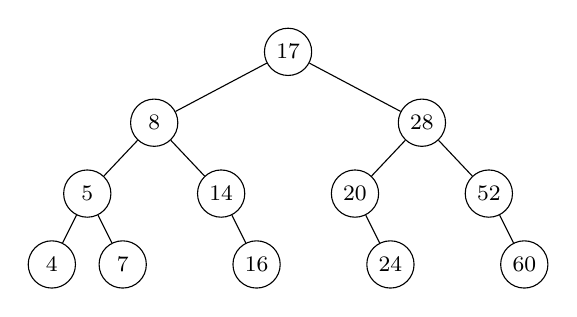
\begin{tikzpicture}[v/.style={circle,draw,minimum size=6mm,inner sep=0pt,font=\footnotesize},
    level distance=9mm, level 1/.style={sibling distance=34mm}, level 2/.style={sibling distance=17mm},
    level 3/.style={sibling distance=9mm}]
\node[v] {17}
  child {node[v] {8} child {node[v] {5} child {node[v] {4}} child {node[v] {7}}}
    child {node[v] {14} child[missing] {} child {node[v] {16}}}}
  child {node[v] {28} child {node[v] {20} child[missing] {} child {node[v] {24}}}
    child {node[v] {52} child[missing] {} child {node[v] {60}}}};
\end{tikzpicture}
\end{center}
檢查：中序是 4, 5, 7, 8, 14, 16, 17, 20, 24, 28, 52, 60（由小到大）；平衡因子 17、8、28、5 是 $0$，14、20、52 是 $-1$，
其餘葉節點 $0$，全部在 $\{-1, 0, +1\}$ 裡。 $12$ 個節點，高度 $3$（數邊）。
\end{pastsoln}
